\documentclass[spanish]{udpreport}
\usepackage[utf8]{inputenc}
\usepackage[spanish]{babel}

% Podemos establecer el logo de alguna entidad o dejar el de la UDP (defecto)
%\setlogo{EITFI}

\title{Informe de redes de datos 5\\
"Montaje y uso de un SWITCH"\\}
\author{Alumno: Camilo Araya
\\Profesor: Nicolás Hidalgo\\Ayudante: Martín Griño}
\date{\today}



\begin{document}
\maketitle

\chapter*{Resumen} 
\addcontentsline{toc}{section}{Resumen} 
\markboth{RESUMEN}{RESUMEN} 
El presente informe tiene por objetivo ser un complemento del informe anterior (stp y vlan), llevando a la practica el montaje de un switch real junto con la configuraciones STP y VLAN respectivamente.
\tableofcontents
\chapter{Introducción}
Hay ocasiones en que en una red implementada existan problemas de congestión debido a la redundancia de esta, los cuales en algunos casos puede generar problemas (ocasionado principalmente por los loops), para ello se tiene que en los Switches existen protocolos con el fin de descongestionar o bien lograr una mejor administración de la red, estos protocolos se mencionaran a continuación:
\section{STP}
Spanning Tree Protocol que en siglas se denomina STP un protocolo de capa 2 que se ejecuta en Bridges y Switches, la especificación es IEEE 802.1D. El objetivo de STP es garantizar que no se creen loops al armar una red que tenga trayectorias redundantes.
\section{VLAN}
Virtual LAN que en siglas es VLAN es un método para crear redes lógicas independientes dentro de una misma red física, el objetivo de esto es aliviar la sobrecarga ejercida en el switch al momento de tener una red con trayectorias redundantes.
\chapter{Desarrollo practico}
Como se menciona anteriormente, esta experiencia se basa fundamentalmente en la configuración de los Switches real con el propósito de implementar los protocolos STP y VLAN, estos cambios que se realizan dentro de la red creada en laboratorio serán en parte para ver de manera practica y sencilla  el funcionamiento de estos dispositivos.
\section{Montaje}
Lo primero que se realizo fue conectar el dispositivo (ilustración 1) a la red (ilustración 2) mediante un cable de red.
\\[0.2cm]
\begin{figure}[h]
    \centering
    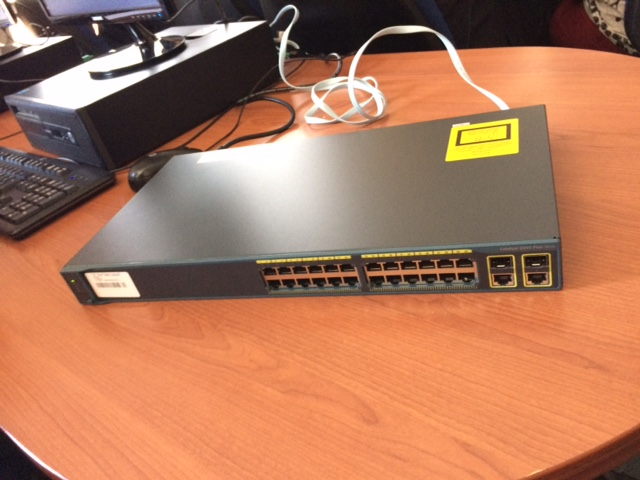
\includegraphics[scale=0.5]{images/a1a1.png}
    \caption{Ilustración 1.}
    \label{fig:my_label}
\end{figure}
\newpage
\begin{figure}[h]
    \centering
    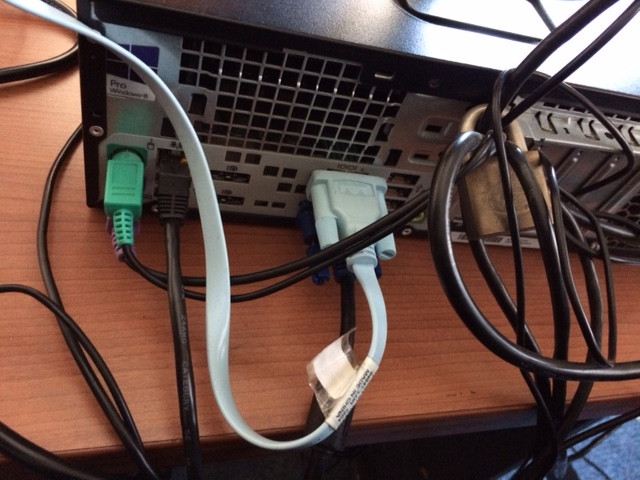
\includegraphics[scale=0.5]{images/a2a2.png}
    \caption{ilustración 2}
    \label{fig:my_label}
\end{figure}
\\[0.2cm]
En esta primera etapa se conectan los respectivos cables uniendo ambos dispositivos, de esta forma se verifica que todo este dispuesto como el ayudante lo requería para no caer en un uso indebido del dispositivo como dañarlo o generar accidentes.
\\[0.2cm]
En cuanto al uso del computador, se procede a abrir la terminal del SO Linux, donde se  realizan los siguientes pasos:
\\
\begin{itemize}
    \item SUDO apt-get install putty(9600 baudios-speed)
    \item Conexión y posterior manipulación del switch.
\end{itemize}

\newpage
\section{Aplicación practica}
Luego de montar nuestra experiencia se procedió a evaluar el funcionamiento del switch, para ello el ayudante nos exigió de modo introductorio generar una tormenta broadcast con el uso de los STP indicados previamente, para ello mediante la consola de linux inhabilitamos y de esta forma el indicador del switch (led de color verde) realizaba parpadeos reiteradas veces, luego de esto se procede posteriormente a realizar las conexiones.
\\[0.2cm]
\begin{figure}[h]
    \centering
    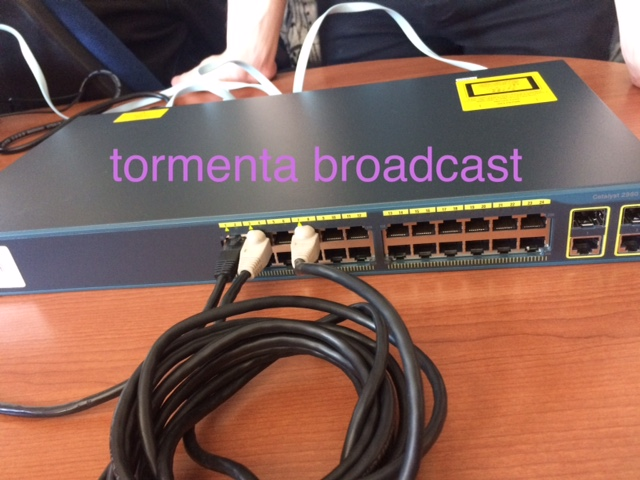
\includegraphics[scale=0.5]{images/a3a3a3.png}
    \caption{ilustración 3.}
    \label{fig:my_label}
\end{figure}
\\[0.2cm]
Lo central de esta actividad fue configurar el equipo que fue proporcionado por el ayudante con la finalidad de configurar el protocolo STP y VLAN tomando como referencia lo realizado en el laboratorio 4, en el cual se hizo uso del simulador Cisco Packet Tracer dichas configuraciones.
\newpage
\subsection{Implementación de protocolos }
Como se especifica anteriormente, esta experiencia es la aplicación practica de lo visto en el laboratorio, esto implica que los códigos proporcionados por el ayudante para la realización de las configuraciones son los mismos que se utilizaran para ingresar a la terminal, los cuales se volverán a mencionar a continuación.
\begin{figure}[h]
    \centering
    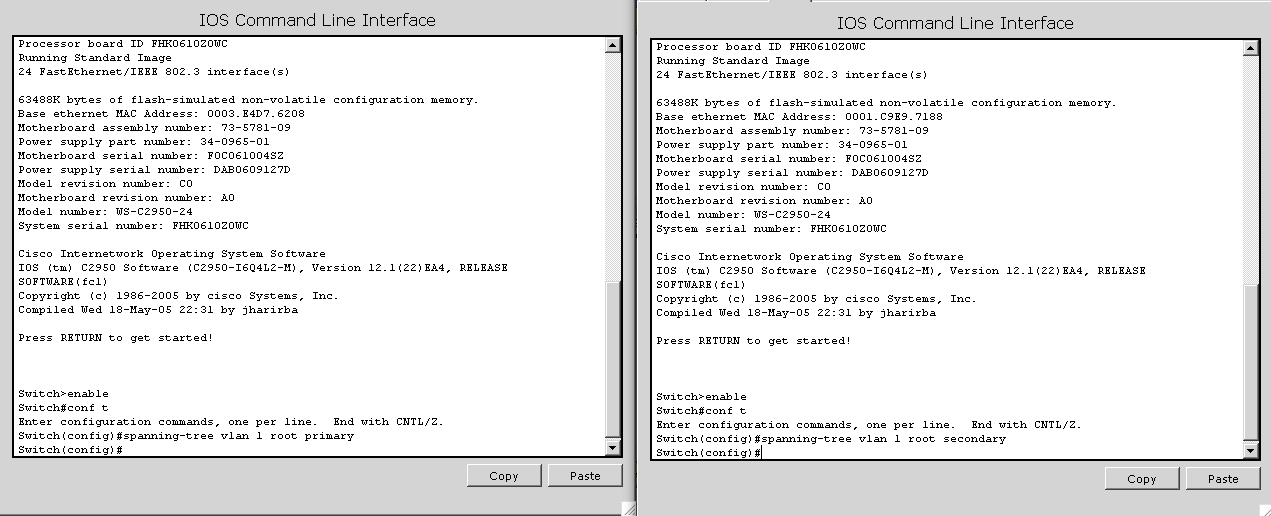
\includegraphics[scale=0.3]{images/cod.png}
    \caption{Protocolo STP}
    \label{fig:my_label}
\end{figure}
\begin{figure}[h]
    \centering
    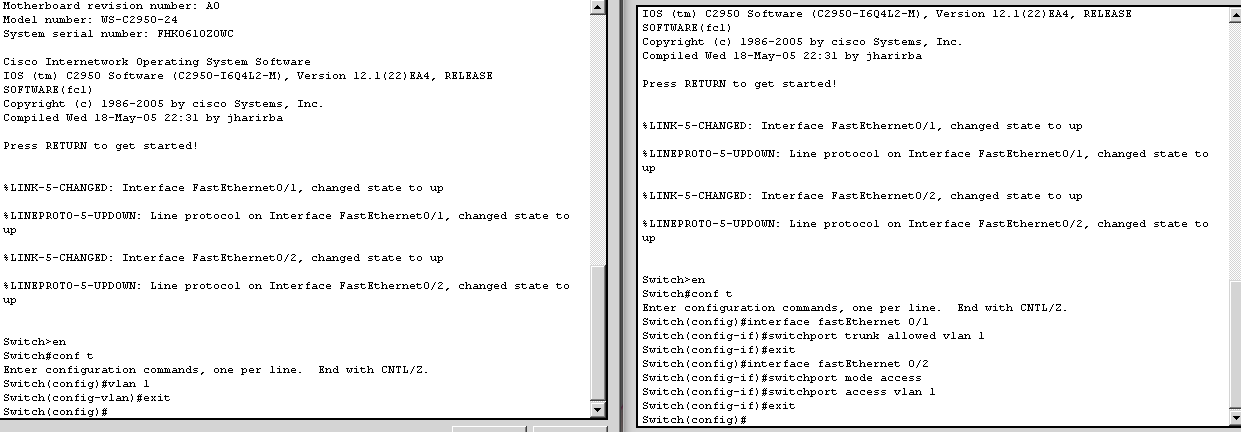
\includegraphics[scale=0.3]{images/3.png}
    \caption{Vlan}
    \label{fig:my_label}
\end{figure}
\\Se realizó una tormenta broadcast al iniciar la conexión al switch, esto se hizo netamente para demostrar si la mala configuración del switch era el responsable de la tormenta de difusión. Posteriormente, junto con el ayudante se fue testeando la implementación de los protocolos STP y VLAN haciando uso de los codigos proporcionados en la \textbf{figura 2.4} y la \textbf{figura 2.5}
\chapter{Conclusión}
Del presente informe se concluye que el trabajo con un Switch Cisco físico en el cual se implementaron los protocolos de Switch STP y VLAN en una red con redundancias, similar a lo visto en la experiencia anterior, solo que ahora lo visto teoricamente se aplico a la practica real. 
\\ Finalmente, se tiene que el conocimiento practico del funcionamiento de estas redes es fundamental para comprender la teoría vista en cátedra sobre STP y VLAN.
\begin{thebibliography}{0}
\bibitem{1}Introducción y configuración de STP. Recuperado de: \\ \url{https://www.cisco.com/c/es_mx/support/docs/lan-switching/spanning-tree-protocol/5234-5.html}
\bibitem{2}que es una VLAN y su funcionamiento. Recuperado de: \\
\url{http://redesconfiguracion.blogspot.cl/2015/07/que-es-una-vlan-y-su-funcion.html}
\end{thebibliography}
\listoffigures
\end{document}

